\renewcommand{\theequation}{\theenumi}
\begin{enumerate}[label=\arabic*.,ref=\thesubsubsection.\theenumi]
\numberwithin{equation}{enumi}
\item The vector form of general equation of circle, 
\begin{align} 
\vec{x}^T\vec{x}-2\vec{O}^T\vec{x}+F=0 \label{eq:circ}
\end{align}
whose centre is $\vec{O}$.

\item Point $\vec{A}$ = $\myvec{4\\1}$ lies on the circle. So, point $A$ satisfies the equation \ref{eq:circ} \\
$\myvec{4\\1}^T\myvec{4\\1}-2\vec{O}^T\myvec{4\\1}+F=0$ \\
\begin{align} 
2\vec{O}^T\myvec{4\\1} - F = 17 \label{eq:circ_1}
\end{align}

\item Point $\vec{B}$ = $\myvec{6\\5}$ lies on the circle. So, point $B$ satisfies the equation \ref{eq:circ} 
\begin{align}
\myvec{6\\5}^T\myvec{6\\5}-2\vec{O}^T\myvec{6\\5}+F=0
\\
2\vec{O}^T\myvec{6\\5} - F = 61 \label{eq:circ_2}
\end{align}

\item  Centre $\vec{O}$ lies on the line $\myvec{4&1}\vec{x}=16$ \\
\begin{align} 
\myvec{4&1}\vec{O}=16 \label{eq:circ_3}
\end{align}

\item Solving equations \ref{eq:circ_1}, \ref{eq:circ_2} and \ref{eq:circ_3} \\
$$ \vec{O} = \myvec{3\\4}, F = 15$$
$\implies$ Equation of the circle is $x^2+y^2-6x-8y+15=0$ \\ 
The vector form is 
$$\vec{x}^T\vec{x}-2\myvec{3&4}\vec{x}+15=0$$

\item The circle in Fig.\ref{fig:circ_1} is generated using the following python code 
\begin{lstlisting}
codes/circle/circle.py
\end{lstlisting}

\begin{figure}[!ht]
\centering
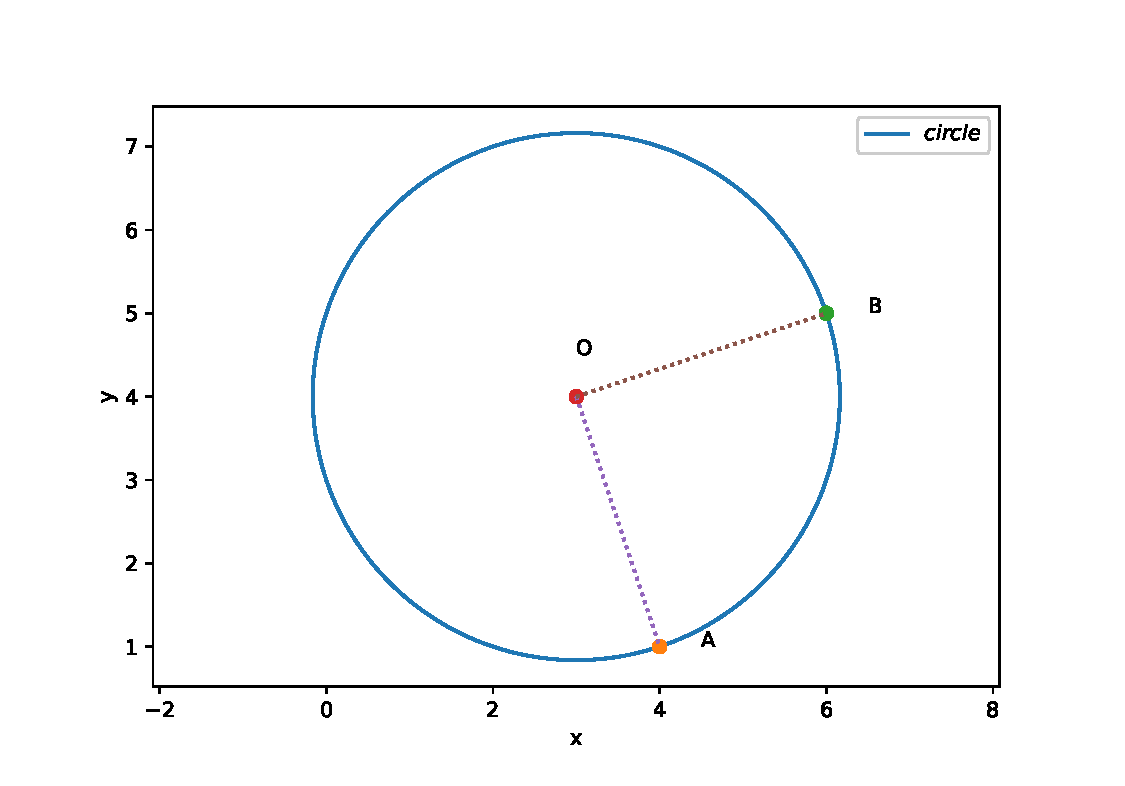
\includegraphics[width=\columnwidth]{./codes/circle/exercise/circle.eps}
\caption{Circle generated using python}
\label{fig:circ_1}
\end{figure}

\end{enumerate}
